\def\code#1{\texttt{#1}}
\makeatletter
Constellation is unique from other systems in its approach of judging the distance of various objects within its captured scene from the camera. Most other approaches might use computationally intensive math and thus have very slow running times. Constellation, instead, uses efficient neural network driven image classification, in combination with simple statistical analysis to perform the same task. The underlying principle which allows this approach to function is that, when refracted through a particularly shaped crystal, the light from a single laser is scattered in such a manner that, as it moves further in distance from its source, it strays further in one direction or the other from its origin. Thus, when it is intercepted by another object at a certain distance, the amount the light at that distance has moved away from the position it would be at if it was intercepted directly in front of the source should be somewhat representative of the numerical distance travelled by that light, and additionally, the distance between individual points of refracted light should also be indicative of the distance from the camera, as each refracted beam of light would stray further from its neighbors.

Constellation's object detection and classification subsystem provides the image coordinates of the center of the object it detects. This is the foundation point used for judging the distance within the image between the laser dots refracted across the figure. In order to find the distance of the object from the camera, the distance between the dots projected onto the object has to be found. Constellation does this by obtaining a sorted list of all the points in the image, a process which in the worst case is $O(n\log n)$, due to the choice to employ a modified Timsort algorithm, but due to the nature of Constellation's object detection implementation, trends nearer to $O(n)$. Following processing and sorting the list of all the dots found in the image, Constellation proceeds to conduct a modified binary search through the list in an effort to find the laser dot closest to the center of the object, taking $O(\log n)$ in both the worst and average cases. Once that has been acquired, the system takes an iterative approach to finding as many possible non-distorted dots on the surface of the object, calculating the euclidean distance between the dot closest to the center of the object and the 4 nearest dots, and checking if they are within the shape of the object determined during the process of training Constellation to recognize the object. If all 4 of the closest dots are within the shape of the object, Constellation proceeds to check the next 4 closest dots, and so on. The entirety of these processes assembles an array of all the representative dots on the visible surface of the object, and that array is used to find the average euclidean distance between each all the points on the surface of the object.

As mentioned earlier, the distance between the refracted dots projected onto an object is theoretically representative of the distance of that object from the camera which captured the image. Several approaches were considered when determining the most efficient and accurate method to extract information about an object's distance from the camera, including finding an as-accurate-as-possible multiple-degree polynomial modeling of the distance between dots vs. the distance from the camera, linear modeling, training a neural network to predict the distance, and a k-nearest neighbors (KNN) approach. Firstly, we considered multiple degree polynomials to mathematically model the correspondence between average distance between dots on the surface of an object and the distance of that object, however, polynomials over a degree of 2  often result in over-fitting, or creating a model which too closely or too accurately represents the training set. This might seem like an advantage of this approach, however, over-fitted models never generalize well to datasets beyond the training set, and thus, as shown in figure 5, actually lose accuracy. So, the rational next step after multiple degree polynomials is linear modeling. A linear function representing the relationship would probably be fairly accurate and abstract well enough to general datasets, however, linear functions exhibit another phenomenon called "underfitting", which means that the model is neither very accurate with the training set nor with general sets. Having ruled out functional modeling all together, the focus was shifted towards models grounded in statistical science and machine learning. Having already heavily implemented them in other parts of Constellation, neural networks were considered for the tasks, but it was determined that they were uneccesary due to their relatively extensive training data necessity and comparatively slow classification speed. Another machine learned based model, SVMs, were considered, but SVMs can only really produce one decision boundary in a dataset well, and therefore cannot be abstracted to classify more than 2 possibilities or labels easily (Weston, Jason, and Chris Watkins, 1998). All of these reasonings led to the choice of a KNN model, a model which finds the $k$ nearest data points to the one which is to be classified, and essentially lets them "vote" on the classification of the data point based on their own classifications, therefore choosing the majority classification of the points near the target point. The graph in figure 5 graphically illustrates the advantages and disadvantages of each of the viable considered models in this particular task on a sample dataset.

\begin{figure}[h]
\centering





\tikzset{every picture/.style={line width=0.75pt}} %set default line width to 0.75pt        

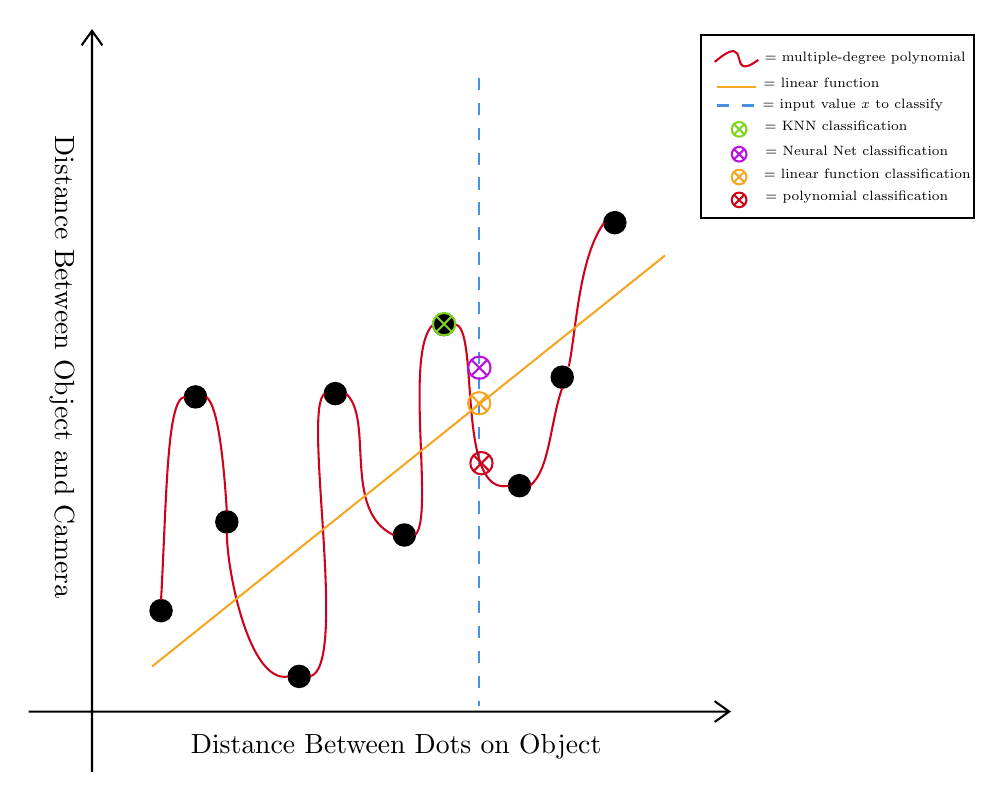
\begin{tikzpicture}[x=0.75pt,y=0.75pt,yscale=-1,xscale=1]
%uncomment if require: \path (0,469); %set diagram left start at 0, and has height of 469

\draw  (50,410) -- (387.5,410)(80.5,82) -- (80.5,439) (380.5,405) -- (387.5,410) -- (380.5,415) (75.5,89) -- (80.5,82) -- (85.5,89)  ;
\draw  [fill={rgb, 255:red, 0; green, 0; blue, 0 }  ,fill opacity=1 ]  (113.77, 361.37) circle [x radius= 5.15, y radius= 5.15]  ;
\draw  [fill={rgb, 255:red, 0; green, 0; blue, 0 }  ,fill opacity=1 ]  (180.31, 393.06) circle [x radius= 5.15, y radius= 5.15]  ;
\draw  [fill={rgb, 255:red, 0; green, 0; blue, 0 }  ,fill opacity=1 ]  (145.45, 318.6) circle [x radius= 5.15, y radius= 5.15]  ;
\draw  [fill={rgb, 255:red, 0; green, 0; blue, 0 }  ,fill opacity=1 ]  (231, 324.93) circle [x radius= 5.15, y radius= 5.15]  ;
\draw  [fill={rgb, 255:red, 0; green, 0; blue, 0 }  ,fill opacity=1 ]  (197.73, 256.81) circle [x radius= 5.15, y radius= 5.15]  ;
\draw  [fill={rgb, 255:red, 0; green, 0; blue, 0 }  ,fill opacity=1 ]  (130.36, 258.39) circle [x radius= 5.15, y radius= 5.15]  ;
\draw  [fill={rgb, 255:red, 0; green, 0; blue, 0 }  ,fill opacity=1 ]  (286.45, 301.17) circle [x radius= 5.15, y radius= 5.15]  ;
\draw  [fill={rgb, 255:red, 0; green, 0; blue, 0 }  ,fill opacity=1 ]  (250.01, 223.54) circle [x radius= 5.15, y radius= 5.15]  ;
\draw  [fill={rgb, 255:red, 0; green, 0; blue, 0 }  ,fill opacity=1 ]  (307.05, 248.89) circle [x radius= 5.15, y radius= 5.15]  ;
\draw  [fill={rgb, 255:red, 0; green, 0; blue, 0 }  ,fill opacity=1 ]  (332.4, 174.43) circle [x radius= 5.15, y radius= 5.15]  ;
\draw [color={rgb, 255:red, 74; green, 144; blue, 226 }  ,draw opacity=1 ] [dash pattern={on 4.5pt off 4.5pt}]  (267.04,104.67) -- (267.04,407.5) ;


\draw [color={rgb, 255:red, 208; green, 2; blue, 27 }  ,draw opacity=1 ]   (113.77,356.22) .. controls (116.5,306) and (116.5,259) .. (125.21,258.39) ;


\draw [color={rgb, 255:red, 208; green, 2; blue, 27 }  ,draw opacity=1 ]   (145.45,323.74) .. controls (145.5,343) and (156.5,397) .. (175.16,393.06) ;


\draw [color={rgb, 255:red, 208; green, 2; blue, 27 }  ,draw opacity=1 ]   (185.46,393.06) .. controls (204.5,389) and (181.5,264) .. (192.58,256.81) ;


\draw [color={rgb, 255:red, 208; green, 2; blue, 27 }  ,draw opacity=1 ]   (202.88,256.81) .. controls (216.5,269) and (200.9,313.45) .. (225.85,324.93) ;


\draw [color={rgb, 255:red, 208; green, 2; blue, 27 }  ,draw opacity=1 ]   (236.15,324.93) .. controls (245.66,317.01) and (230.5,236) .. (244.87,223.54) ;


\draw [color={rgb, 255:red, 208; green, 2; blue, 27 }  ,draw opacity=1 ]   (255.16,223.54) .. controls (267.5,223) and (255.5,307) .. (281.3,301.17) ;


\draw [color={rgb, 255:red, 208; green, 2; blue, 27 }  ,draw opacity=1 ]   (291.6,301.17) .. controls (301.11,293.25) and (301.11,271.07) .. (307.05,254.04) ;


\draw [color={rgb, 255:red, 208; green, 2; blue, 27 }  ,draw opacity=1 ]   (310.22,243.74) .. controls (313.78,226.71) and (314.97,191.46) .. (327.25,174.43) ;


\draw [color={rgb, 255:red, 245; green, 166; blue, 35 }  ,draw opacity=1 ]   (109.41,388.3) -- (356.56,190.27) ;


\draw [color={rgb, 255:red, 208; green, 2; blue, 27 }  ,draw opacity=1 ]   (145.45,313.45) .. controls (142.5,265) and (137.5,260) .. (135.51,258.39) ;


\draw  [color={rgb, 255:red, 126; green, 211; blue, 33 }  ,draw opacity=1 ] (244.76,223.32) .. controls (244.76,220.36) and (247.17,217.95) .. (250.13,217.95) .. controls (253.1,217.95) and (255.5,220.36) .. (255.5,223.32) .. controls (255.5,226.28) and (253.1,228.69) .. (250.13,228.69) .. controls (247.17,228.69) and (244.76,226.28) .. (244.76,223.32) -- cycle ; \draw  [color={rgb, 255:red, 126; green, 211; blue, 33 }  ,draw opacity=1 ] (246.34,219.52) -- (253.93,227.12) ; \draw  [color={rgb, 255:red, 126; green, 211; blue, 33 }  ,draw opacity=1 ] (253.93,219.52) -- (246.34,227.12) ;
\draw  [color={rgb, 255:red, 245; green, 166; blue, 35 }  ,draw opacity=1 ] (261.68,261.45) .. controls (261.68,258.49) and (264.08,256.08) .. (267.04,256.08) .. controls (270.01,256.08) and (272.41,258.49) .. (272.41,261.45) .. controls (272.41,264.41) and (270.01,266.82) .. (267.04,266.82) .. controls (264.08,266.82) and (261.68,264.41) .. (261.68,261.45) -- cycle ; \draw  [color={rgb, 255:red, 245; green, 166; blue, 35 }  ,draw opacity=1 ] (263.25,257.65) -- (270.84,265.25) ; \draw  [color={rgb, 255:red, 245; green, 166; blue, 35 }  ,draw opacity=1 ] (270.84,257.65) -- (263.25,265.25) ;
\draw  [color={rgb, 255:red, 208; green, 2; blue, 27 }  ,draw opacity=1 ] (262.76,290.32) .. controls (262.76,287.36) and (265.17,284.95) .. (268.13,284.95) .. controls (271.1,284.95) and (273.5,287.36) .. (273.5,290.32) .. controls (273.5,293.28) and (271.1,295.69) .. (268.13,295.69) .. controls (265.17,295.69) and (262.76,293.28) .. (262.76,290.32) -- cycle ; \draw  [color={rgb, 255:red, 208; green, 2; blue, 27 }  ,draw opacity=1 ] (264.34,286.52) -- (271.93,294.12) ; \draw  [color={rgb, 255:red, 208; green, 2; blue, 27 }  ,draw opacity=1 ] (271.93,286.52) -- (264.34,294.12) ;
\draw  [color={rgb, 255:red, 189; green, 16; blue, 224 }  ,draw opacity=1 ] (261.76,244.32) .. controls (261.76,241.36) and (264.17,238.95) .. (267.13,238.95) .. controls (270.1,238.95) and (272.5,241.36) .. (272.5,244.32) .. controls (272.5,247.28) and (270.1,249.69) .. (267.13,249.69) .. controls (264.17,249.69) and (261.76,247.28) .. (261.76,244.32) -- cycle ; \draw  [color={rgb, 255:red, 189; green, 16; blue, 224 }  ,draw opacity=1 ] (263.34,240.52) -- (270.93,248.12) ; \draw  [color={rgb, 255:red, 189; green, 16; blue, 224 }  ,draw opacity=1 ] (270.93,240.52) -- (263.34,248.12) ;
\draw    (374, 84) rectangle (505.5, 172)   ;
\draw [color={rgb, 255:red, 208; green, 2; blue, 27 }  ,draw opacity=1 ]   (380.5,97) .. controls (399.5,81) and (385.5,108) .. (401.5,96) ;


\draw [color={rgb, 255:red, 245; green, 166; blue, 35 }  ,draw opacity=1 ]   (381.5,109) -- (400.5,109) ;


\draw  [color={rgb, 255:red, 126; green, 211; blue, 33 }  ,draw opacity=1 ] (388.76,129.48) .. controls (388.76,127.53) and (390.34,125.95) .. (392.29,125.95) .. controls (394.23,125.95) and (395.81,127.53) .. (395.81,129.48) .. controls (395.81,131.42) and (394.23,133) .. (392.29,133) .. controls (390.34,133) and (388.76,131.42) .. (388.76,129.48) -- cycle ; \draw  [color={rgb, 255:red, 126; green, 211; blue, 33 }  ,draw opacity=1 ] (389.8,126.98) -- (394.78,131.97) ; \draw  [color={rgb, 255:red, 126; green, 211; blue, 33 }  ,draw opacity=1 ] (394.78,126.98) -- (389.8,131.97) ;
\draw  [color={rgb, 255:red, 189; green, 16; blue, 224 }  ,draw opacity=1 ] (388.76,141.48) .. controls (388.76,139.53) and (390.34,137.95) .. (392.29,137.95) .. controls (394.23,137.95) and (395.81,139.53) .. (395.81,141.48) .. controls (395.81,143.42) and (394.23,145) .. (392.29,145) .. controls (390.34,145) and (388.76,143.42) .. (388.76,141.48) -- cycle ; \draw  [color={rgb, 255:red, 189; green, 16; blue, 224 }  ,draw opacity=1 ] (389.8,138.98) -- (394.78,143.97) ; \draw  [color={rgb, 255:red, 189; green, 16; blue, 224 }  ,draw opacity=1 ] (394.78,138.98) -- (389.8,143.97) ;
\draw  [color={rgb, 255:red, 245; green, 166; blue, 35 }  ,draw opacity=1 ] (388.76,152.48) .. controls (388.76,150.53) and (390.34,148.95) .. (392.29,148.95) .. controls (394.23,148.95) and (395.81,150.53) .. (395.81,152.48) .. controls (395.81,154.42) and (394.23,156) .. (392.29,156) .. controls (390.34,156) and (388.76,154.42) .. (388.76,152.48) -- cycle ; \draw  [color={rgb, 255:red, 245; green, 166; blue, 35 }  ,draw opacity=1 ] (389.8,149.98) -- (394.78,154.97) ; \draw  [color={rgb, 255:red, 245; green, 166; blue, 35 }  ,draw opacity=1 ] (394.78,149.98) -- (389.8,154.97) ;
\draw  [color={rgb, 255:red, 208; green, 2; blue, 27 }  ,draw opacity=1 ] (388.76,163.48) .. controls (388.76,161.53) and (390.34,159.95) .. (392.29,159.95) .. controls (394.23,159.95) and (395.81,161.53) .. (395.81,163.48) .. controls (395.81,165.42) and (394.23,167) .. (392.29,167) .. controls (390.34,167) and (388.76,165.42) .. (388.76,163.48) -- cycle ; \draw  [color={rgb, 255:red, 208; green, 2; blue, 27 }  ,draw opacity=1 ] (389.8,160.98) -- (394.78,165.97) ; \draw  [color={rgb, 255:red, 208; green, 2; blue, 27 }  ,draw opacity=1 ] (394.78,160.98) -- (389.8,165.97) ;
\draw [color={rgb, 255:red, 74; green, 144; blue, 226 }  ,draw opacity=1 ] [dash pattern={on 4.5pt off 4.5pt}]  (381.5,118) -- (400.5,118) ;



\draw (66,244) node [rotate=-90] [align=left] {Distance Between Object and Camera};
\draw (227,427) node  [align=left] {Distance Between Dots on Object};
\draw (453,95) node [scale=0.7] [align=left] {{\scriptsize = multiple-degree polynomial}};
\draw (432,107) node [scale=0.7] [align=left] {{\scriptsize = linear function}};
\draw (439,128) node [scale=0.7] [align=left] {{\scriptsize = KNN classification}};
\draw (449,140) node [scale=0.7] [align=left] {{\scriptsize = Neural Net classification}};
\draw (454,151) node [scale=0.7] [align=left] {{\scriptsize = linear function classification}};
\draw (449,162) node [scale=0.7] [align=left] {{\scriptsize = polynomial classification}};
\draw (447,118) node [scale=0.7] [align=left] {{\scriptsize = input value \textit{x} to classify}};


\end{tikzpicture}

\caption{Different Classification Approaches on Sample Set}
\end{figure}

A KNN model's accuracy grows near-exponentially with the addition of more labeled training data, as its training data is essentially the entire model. Constellation currently operates on limited range, due in part to the limited visibility of the laser dots as they move farther from the source, but also due to the limitation of available training data. As of now, a relatively large training set with over \begin{it}x\end{it} data points has been gathered, and is effectively used to predict distance within a range of \begin{it}x\end{it}. As described earlier, the model predicts the distance of an object depending on the spread of the laser dots on the object's surface by finding the values of the 6 nearest data points and letting them vote on an appropriate distance for the object. Assume there is a defined function \texttt{majority\_vote(labels)} which returns the majority vote of $k$ labels and, in the case of ties, recursively reduces $k$ until there are no more ties. Given that, the following is an abridged psuedocode segment of Constellation's implementation of a KNN model illustrating the logic behind the model:
\def\BState{\State\hskip-\ALG@thistlm}
\begin{algorithm}
\caption{KNN Classification Algorithm}\label{euclid}
\begin{algorithmic}[1]
\Procedure{knn\_classify(k, labeled points, new point):}{}
\State $\text{by distance}\gets\text{sorted labeled points by distance from new point}$
\State $\text{create empty list of k nearest}$
\State $\emph{loop} \text{ for first }$k$\text{ points in by distance:}$ %
\State $\enspace\enspace\text{k nearest}\gets\text{k nearest}+\text{point}$
\State $\text{classification}\gets\text{majority\_vote(k nearest)}$
\State $\Return \text{ classification}$
\EndProcedure
\end{algorithmic}
\end{algorithm}